\section{Results}
\label{sec:results}

Results are reported in four parts. The first is how the detectors perform on clean
data, which fixes the baseline. The second is how they perform against the transmitted
attacks. The third follows one missed attack into the navigation solution. The fourth
compares these measurements against what a perturbation of the measurements alone would
have suggested.

\subsection{Clean performance and false alarm cost}
\label{sec:res_clean}

Every detector is set to the common operating point of Equation~\ref{eq:oppoint}, which
is the highest threshold at which it still flags 95 percent of the spoofed samples in
clean validation data. Table~\ref{tab:main} reports what each detector achieves there.

Two quantities describe clean performance. The $F_1$ score is the harmonic mean of
precision and recall, so it summarises detection quality in one number. The false alarm
rate is the fraction of authentic samples the detector flags, and it is the cost of
meeting the recall floor.

\begin{table*}[t]
\centering
\caption{Every detector at the common operating point of Equation~\ref{eq:oppoint},
ordered by false alarm rate. Passed counts the transmitted take over attacks, out of
126, for which the detector flags fewer than half the spoofed samples. Lowest detection
is the smallest fraction of an attack's samples the detector flagged. The final column
is the smallest perturbation of the measurements alone that crosses the decision
boundary, for comparison.}
\label{tab:main}
\footnotesize
\begin{tabular}{@{}llrrrrr@{}}
\toprule
 & & \multicolumn{2}{c}{Clean data} & \multicolumn{2}{c}{Transmitted attacks}
 & Perturbation \\
\cmidrule(lr){3-4}\cmidrule(lr){5-6}\cmidrule(lr){7-7}
Detector & Family & $F_1$ & False alarm & Passed & Lowest det.
 & $L_\infty$ \\
\midrule
Random forest & classical & 0.833 & 0.337 & 55 (43.7\%) & 0.001 & 0.025 \\
Gradient boosting & classical & 0.827 & 0.350 & 27 (21.4\%) & 0.166 & 0.019 \\
Temporal convolutional & deep & 0.805 & 0.427 & 4 (3.2\%) & 0.469 & 0.041 \\
XGBoost & classical & 0.811 & 0.451 & 28 (22.2\%) & 0.088 & 0.020 \\
Nearest neighbour & classical & 0.800 & 0.462 & 0 (0.0\%) & 0.692 & 0.055 \\
LightGBM & classical & 0.804 & 0.464 & 27 (21.4\%) & 0.151 & 0.021 \\
Decision tree & classical & 0.787 & 0.522 & 21 (16.7\%) & 0.139 & 0.023 \\
Multilayer perceptron & classical & 0.758 & 0.587 & 14 (11.1\%) & 0.171 & 0.039 \\
Bidirectional LSTM & deep & 0.741 & 0.662 & 0 (0.0\%) & 0.712 & 0.064 \\
Long short term memory & deep & 0.735 & 0.679 & 0 (0.0\%) & 0.568 & 0.065 \\
Convolutional recurrent & deep & 0.734 & 0.693 & 0 (0.0\%) & 0.725 & 0.067 \\
Convolutional network & deep & 0.725 & 0.737 & 0 (0.0\%) & 0.636 & 0.058 \\
Transformer & deep & 0.707 & 0.794 & 18 (14.3\%) & 0.004 & 0.058 \\
Support vector machine & classical & 0.682 & 0.960 & 53 (42.1\%) & 0.074 & 0.111 \\
\bottomrule
\end{tabular}
\end{table*}

The random forest achieves the highest $F_1$ score at 0.833 and the lowest false alarm
rate at 0.337. Gradient boosting follows at 0.827 and 0.350. The support vector machine
is last on both counts, at 0.682 and 0.960.

The false alarm rates deserve attention on their own. Across the fourteen detectors they
run from 0.337 to 0.960. Even the best of them flags about a third of authentic samples
as spoofed. On this evidence no detector in the study is usable as a standalone
single epoch integrity monitor, before any attacker is considered. A fielded monitor
would combine decisions over several epochs, trading detection latency for a lower rate
of false alarms, and the per epoch numbers reported here are the input to such a scheme.
Figure~\ref{fig:oppoint} shows the clean scores at that operating point.

% Figure source: figures_src/fig_legacy.py
\begin{figure}[t]
\centering
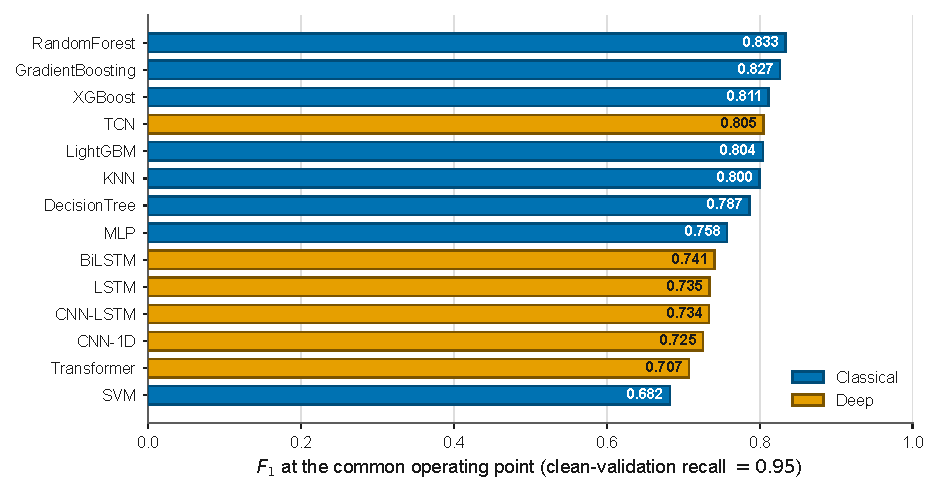
\includegraphics[width=\linewidth]{figures/fig05_detection_operating_point.pdf}
\caption{Clean $F_1$ for every detector at the common operating point, the threshold at which each flags 95 percent of spoofed samples in clean validation data. Classical and deep detectors are interleaved, so no family dominates before an attacker is considered.}
\label{fig:oppoint}
\end{figure}

\subsection{Detector performance under transmitted attacks}
\label{sec:res_attack}

Each detector is then run against the 126 transmitted settings that meet the conditions
for taking over a receiver. For each setting the detection rate is the fraction of that
attack's spoofed samples the detector flags. Because every sample in these files is
spoofed, the detection rate is the detector's recall against that particular attack. A
setting counts as passed when the detector flags fewer than half of its samples.

Table~\ref{tab:main} and Figure~\ref{fig:detection} report the outcome.

\begin{figure}[t]
\centering
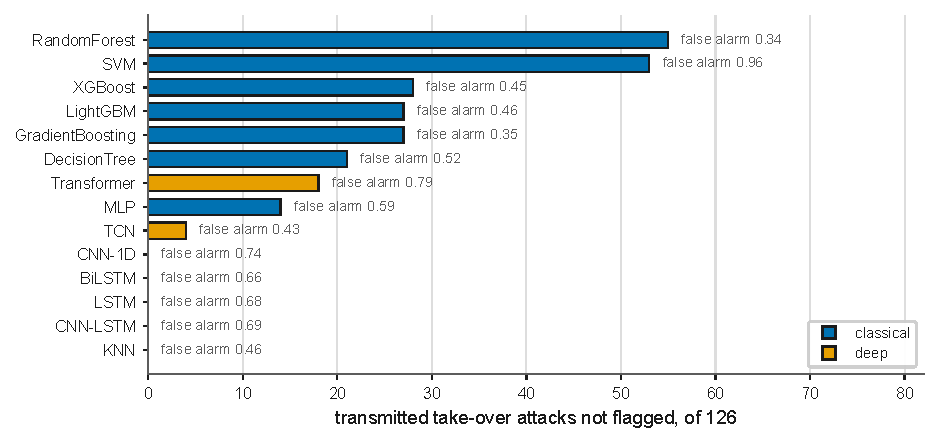
\includegraphics[width=\linewidth]{figures/fig_detection_vs_transmitted.pdf}
\caption{Transmitted take over attacks each detector fails to flag, out of 126. The
clean false alarm rate each detector pays at the common operating point is printed
beside its bar. The detector with the lowest false alarm rate fails to flag the most
attacks.}
\label{fig:detection}
\end{figure}

The detector that performs best on clean data is the one most often passed. The random
forest fails to flag 55 of the 126 attacks, which is 43.7 percent of them. Against one
setting it flags 0.1 percent of the spoofed samples, so the attack is present throughout
and the detector reports authentic almost everywhere.

Gradient boosting fails to flag 27, XGBoost 28 and LightGBM 27. The support vector
machine fails to flag 53, and it does so while flagging 96 percent of authentic samples,
so it is neither accurate nor resistant.

Five detectors flag every one of the 126 attacks. They are the nearest neighbour
classifier, the one dimensional convolutional network, the convolutional recurrent
hybrid, the bidirectional long short term memory and the long short term memory. Their
lowest detection rate against any attack stays between 0.568 and 0.725. Their false alarm
rates on authentic data run from 0.462 to 0.737, so between 46 and 74 percent of
authentic samples are flagged as attacks. Their resistance is bought by flagging a large
part of the authentic data, which is the trade described in
Section~\ref{sec:rw_adversarial} and not a property that could be used in a receiver.

Taken together, no detector in the study is both usable and resistant. The two with the
lowest false alarm rates are passed by 43.7 and 21.4 percent of the attacks. The five
that are never passed carry false alarm rates that rule them out.
Figure~\ref{fig:integrity} places the detectors on the two axes an integrity monitor trades.

% Figure source: figures_src/fig_legacy.py
\begin{figure}[t]
\centering
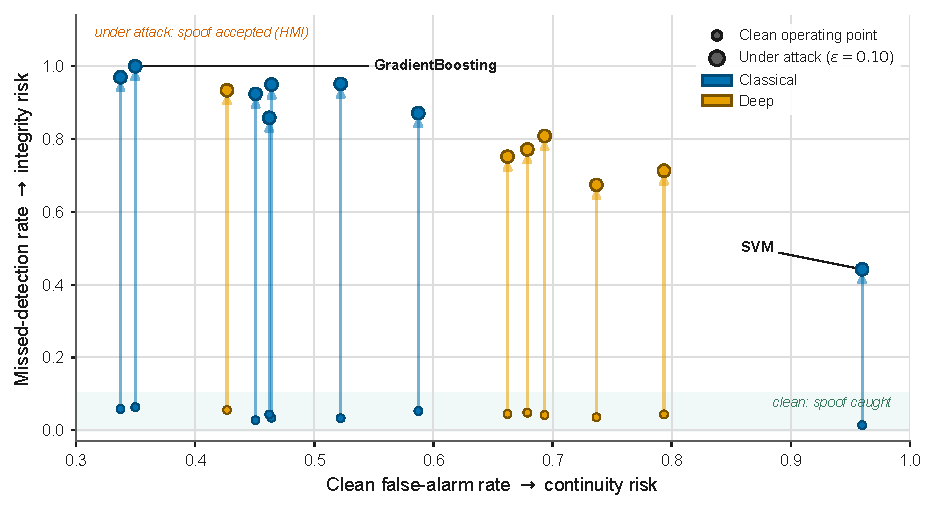
\includegraphics[width=\linewidth]{figures/fig12_integrity_plane.pdf}
\caption{Each detector placed by the two risks a navigation integrity monitor trades. The horizontal axis is the false alarm rate on authentic data, which drives continuity risk. The vertical axis is the missed detection rate, which drives integrity risk. No detector reaches the lower left corner.}
\label{fig:integrity}
\end{figure}

\subsection{A single transmitter setting evading six detectors}
\label{sec:res_single}

The counts above describe an attacker that transmits every setting in turn. A real
attacker chooses one setting and transmits it. The relevant question is therefore what a
single choice achieves.

The best single setting is a counterfeit three decibels stronger than the authentic
signal, in phase with it, dragging the code at 14.65 metres per second. Transmitted once,
it is passed by six of the fourteen detectors at the same time. Those six are the
decision tree, the random forest, gradient boosting, XGBoost, LightGBM and the
Transformer, so every tree based detector in the study is among them, including the one
with the best clean performance, which flags 1.2 percent of the samples.

This is the same setting that Section~\ref{sec:res_nav} follows through the navigation
stage. One transmitted configuration therefore passes six detectors and drives the
receiver clock at the commanded rate. The attacker needs no knowledge of which detector
is running, because this single choice covers six of them.

A second setting, identical except that the code is dragged at 2.93 metres per second,
passes the same six detectors. The attacker can therefore trade the speed of the induced
error against nothing at all, since both rates pass the same set.

\subsection{Navigation domain consequence}
\label{sec:res_nav}

Detection failure matters only if the attack it misses does something. One of the missed
settings is therefore followed through the navigation stage, which is the part of the
receiver that turns the measurements into a position and a clock estimate.

The setting is a counterfeit three decibels stronger than the authentic signal, dragging
the code at 14.65 metres per second. The random forest flags 1.2 percent of its samples.
The attack drags every satellite by the same amount, and a stationary receiver absorbs a
common change in range into its clock estimate, so the expected effect is a drift of the
receiver clock at
\begin{equation}
\frac{\dot\tau \, c/f_\mathrm{chip}}{c} = \frac{14.65}{c} = 48.87~\mathrm{ns/s}.
\label{eq:clockrate}
\end{equation}

The receiver's own clock drift is measured first, by running the same window with the
counterfeit switched off. It is 0.12 nanoseconds per second, so it is negligible against
the rates under test, and it is subtracted from every figure below.

The corrected drift is 48.89 nanoseconds per second against a commanded 48.87, a
difference of 0.02 nanoseconds per second, or 0.05 percent. Figure~\ref{fig:clock} shows the clock
estimate over the window together with the commanded rate. The navigation solution
converged at every epoch with a figure of merit below one metre, so the receiver was
producing an ordinary fix while its clock was being driven.

\begin{figure*}[t]
\centering
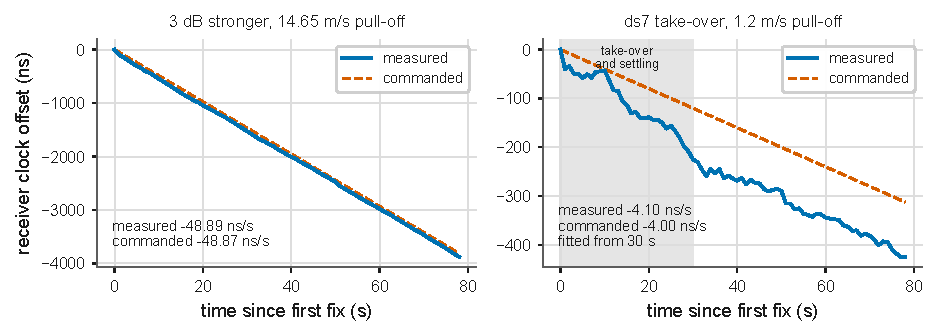
\includegraphics[width=\textwidth]{figures/fig_clock_push.pdf}
\caption{The attack reaches the navigation solution. Receiver clock offset over the
window for two transmitted attacks, with the rate each transmitter was set to impose. In
the left panel the measured drift is within 0.05 percent of the commanded rate. The
detector with the best clean performance reports 98.8 percent of the samples in that
attack as authentic.}
\label{fig:clock}
\end{figure*}

The right panel of Figure~\ref{fig:clock} shows the ds7 takeover at 1.2 metres per
second. This attack carries a takeover of 20 seconds before its code begins to drift, and
the tracking loops need time to settle once they have been captured. Fitting across the
whole window therefore mixes the settling transient with the drift. The measured slope
over successive 20 second segments is $-6.27$, $-7.50$, $-4.72$ and $-4.68$ nanoseconds
per second, so the loops have settled about 30 seconds in.

Fitted after settling, the corrected drift is 4.10 nanoseconds per second against a
commanded 4.00, a difference of 2.3 percent. Both attacks therefore drive the receiver
clock at the rate the transmitter was set to impose, one of them through a takeover and
one without.
Figure~\ref{fig:ladder} sets out what each kind of attack is assumed to know.

% Figure source: figures_src/static/fig_threat_ladder.png (hand made)
\begin{figure*}[t]
\centering
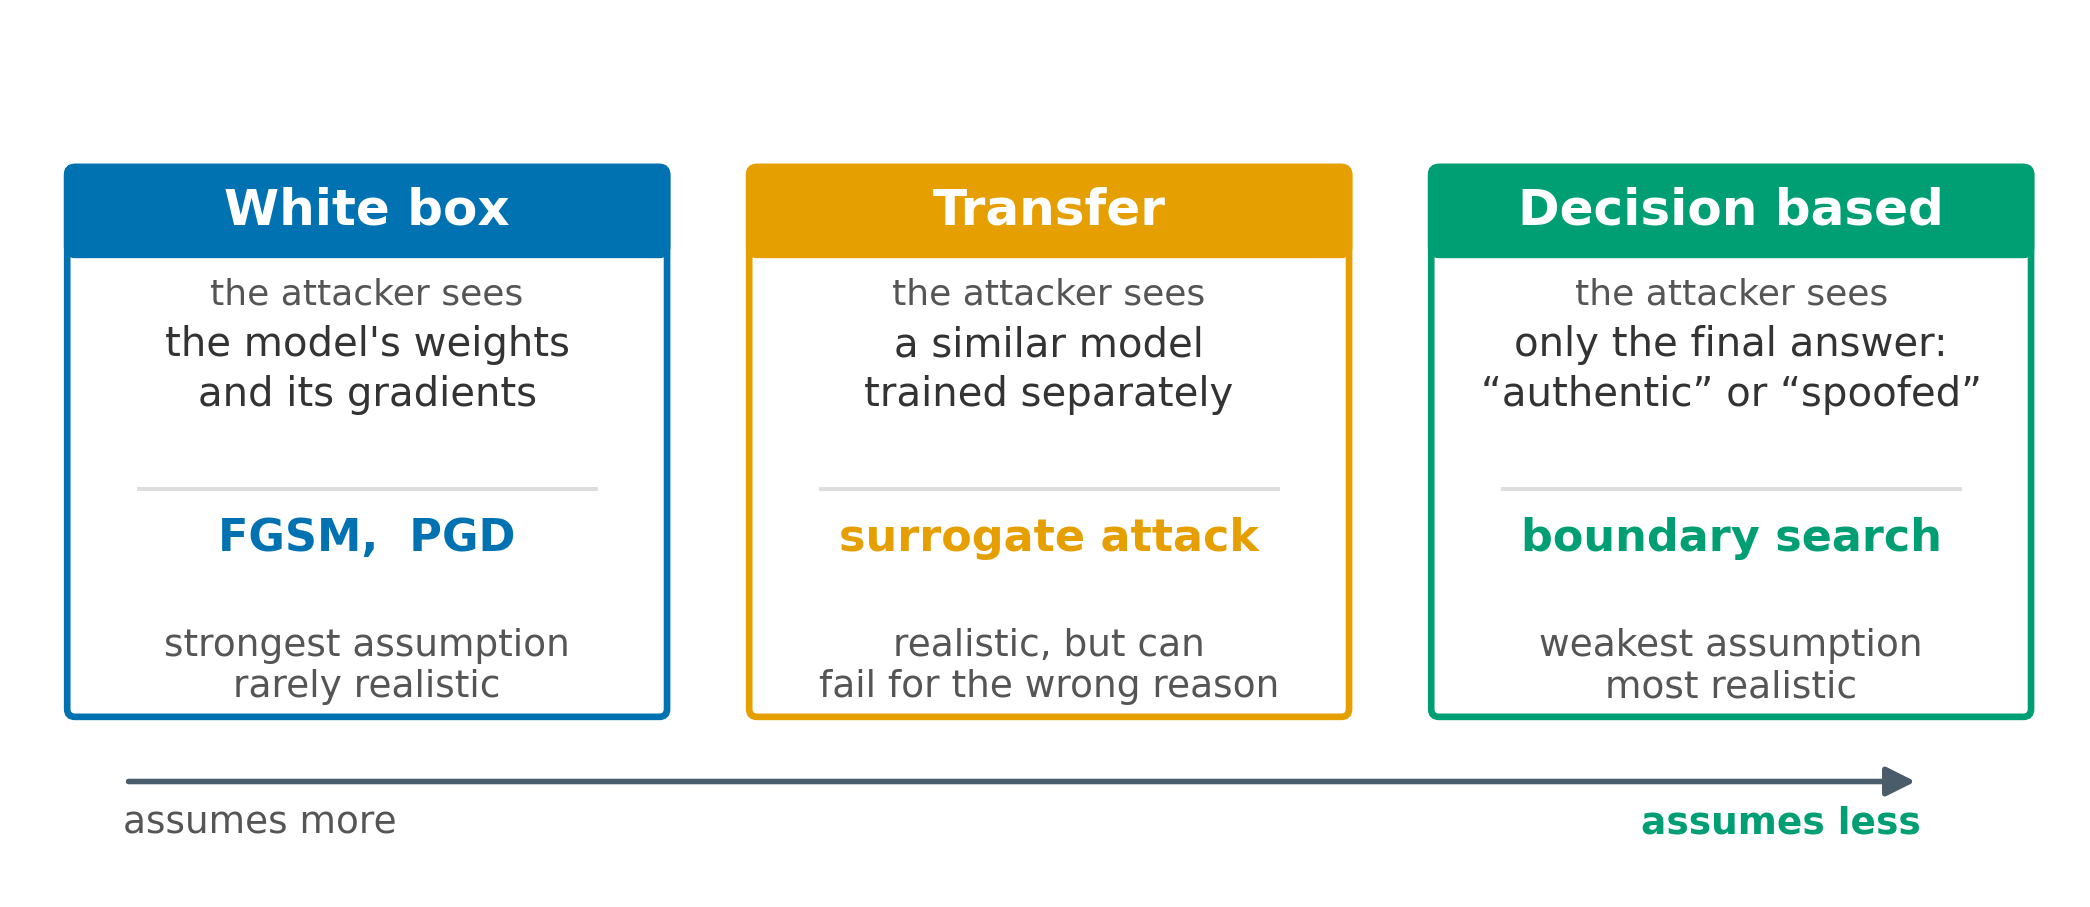
\includegraphics[width=\textwidth]{figures/fig_threat_ladder.png}
\caption{What an attacker is assumed to know. A white box attacker holds the model and its gradients, a transfer attacker holds a separately trained substitute, and a decision based attacker sees only the output decision. The comparison in this section uses the last of these, which assumes least.}
\label{fig:ladder}
\end{figure*}

\subsection{Comparison with feature space evaluation}
\label{sec:res_compare}

The same fourteen detectors were also measured with the decision based boundary attack of
Section~\ref{sec:comparison}, which perturbs the measurements directly without generating
a signal. Table~\ref{tab:main} reports the size of the smallest perturbation that crosses
each detector's decision boundary, expressed in the normalised measurement space.

The two views agree on which detectors are fragile. The tree based detectors need the
smallest perturbations, from 0.019 to 0.025, and they are also the detectors most often
passed by a transmitted attack. The agreement is useful, because it shows the fragility
is a property of those detectors and not an artefact of either measurement.

The two views disagree on the support vector machine. It needs by far the largest
perturbation at 0.111, which taken alone would read as the most robust detector in the
study. Its false alarm rate of 0.960 explains this. A detector that flags almost
everything is hard to push into flagging, and the transmitted measurement shows the same
detector being passed by 53 of the 126 attacks. Reading the perturbation size without the
false alarm rate would have inverted the conclusion.
Figure~\ref{fig:fragility} gives the resulting ranking.

% Figure source: figures_src/fig_legacy.py
\begin{figure}[t]
\centering
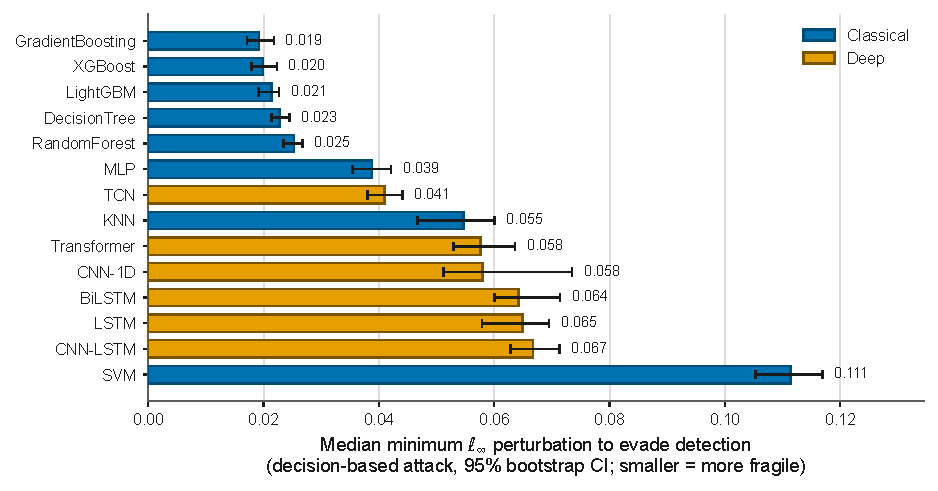
\includegraphics[width=\linewidth]{figures/fig06_fragility_ranking.pdf}
\caption{Median smallest perturbation of the measurements alone that moves each detector across its decision boundary, under the decision based attack. Larger is more resistant. This is the comparison measurement, not the transmitted attack.}
\label{fig:fragility}
\end{figure}
Figure~\ref{fig:rankinv} compares that ranking against the clean one.

% Figure source: figures_src/fig_legacy.py
\begin{figure}[t]
\centering
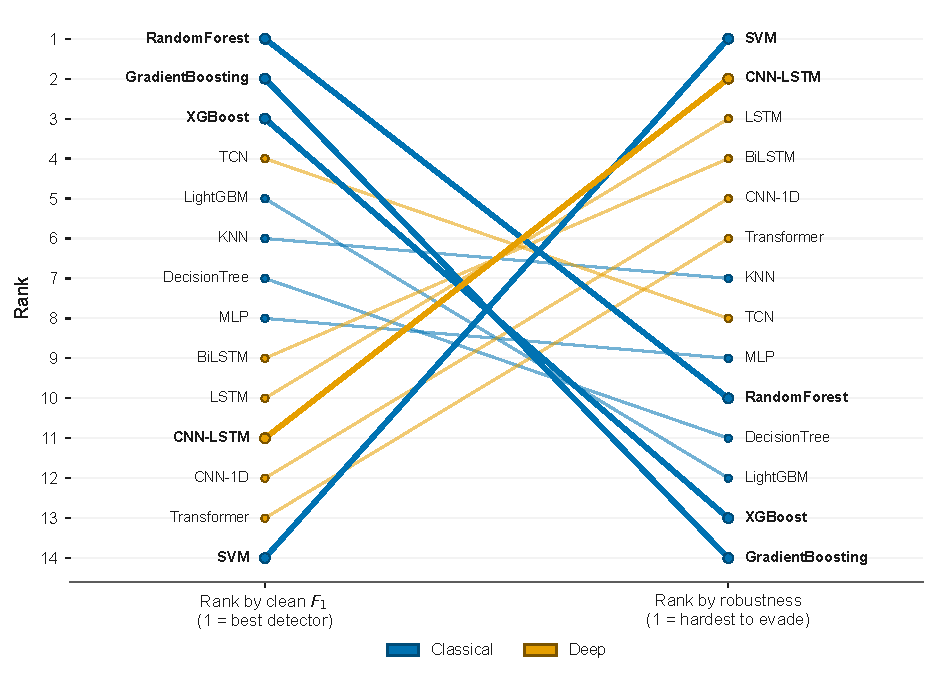
\includegraphics[width=\linewidth]{figures/fig10_rank_inversion.pdf}
\caption{Detectors ranked by clean $F_1$ against the same detectors ranked by resistance to the decision based attack. The two orderings run close to opposite, which is the same relation the transmitted attacks produce.}
\label{fig:rankinv}
\end{figure}
